\newpage

\rhead{\'ECOULEMENTS DIPHASIQUES}
\lhead{Front-Tracking IJK}

\chapter{Front-Tracking IJK}
\label{sec:IJK}

\section{Pr\'esentation du mod\`ele}

The IJK module in TrioCFD relies on the \textit{Front-Tracking discontinu} module for all the FT mesh management. IJK (reference to the three components of a Cartesian coordinate system) is optimized for direct numerical simulations in parallelepipedic domains, discretized on a structured Cartesian grid. Its simplified vectorization allows significant performance gains, in particular thanks to the multigrid solver for the resolution of the pressure. This module is used to perform channel flow calculations (wall boundary conditions available in the z direction), as well as periodic calculations. The periodicity for the Front-Tracking interfaces is ensured with specific algorithm, and allows to study stationary states. The IJK Front-Tracking module is mature for adiabatic calculations of bubbly flows. Front-Tracking IJK is specially designed for bubbly flow studies (neither free surfaces, nor droplets) at low void fraction (<10\%). To date, there is no model for fragmentation, coalescence or wall boiling.

\begin{itemize}
\item Small parallelepipedic domain.
\item At least two periodicity directions (x,y): ideal for stationary states studies.
\item Ideal for adiabatic flows at low void fraction.
\end{itemize}

\subsection{M\'ethode num\'erique}

The Front-Tracking IJK module of TrioCFD resolves the one-fluid equations of ~\cite{kataoka1986} as written for channel up-flow by \cite{lu2008}. Following the proposal of Tryggvason, a front-tracking method is used to solve the set of equations in the whole computational domain, including both the gas and liquid phases. The interface is followed by connected marker points. The Lagrangian markers are advected by the velocity field interpolated from the Eulerian grid. In order to preserve the mesh quality and to limit the need for a smoothing algorithm, only the normal component of the velocity field is used in the marker transport. After transport, the front is used to update the phase indicator function, the density and the viscosity at each Eulerian grid point. The Navier–Stokes equations are then solved by a projection method \cite{puckett1997} using fourth order central differentiation for evaluation of the convective and diffusive terms on a fixed, staggered Cartesian grid. Fractional time stepping leads to a third-order Runge–Kutta scheme \cite{williamson1980}. In the two-step prediction–correction algorithm, a surface tension source is added to the main flow source term and to the evaluation of the convection and diffusion operators in order to obtain the predicted velocity (see \cite{mathieu2003} for further information). Then, an elliptic pressure equation is solved by an algebraic multigrid method to impose a divergence-free velocity field.

\subsection{Périodicité pour les écoulements cisaillés}

La condition de shear-periodicité consiste à imposer à la frontière $\partial\omega_z$ une condition de périodicité accompagnée d'un saut de vitesse. Pour imposer un écoulement cisaillé linéaire moyen $U\lrb{z}=Sz$~\cite{tanaka2015,tanaka2017,rosti2019}, le saut de vitesse au bord $\partial\omega_z$ est $\lrbb{\lrbb{U}}_{\partial\omega_z}=SL_z$. L'intégration de cette condition de saut en temps permet d'obtenir le décalage spatial $\lrbb{\lrbb{X}}_{\partial\omega_z}=SL_zt$. Ainsi, la tri-périodicité d'un domaine (avec condition de shear-periodicité selon z), s'écrit :

\begin{align}
\phi\lrb{x+L_x,y,z}&=\phi\lrb{x,y,z}\\
\phi\lrb{x,y+L_y,z}&=\phi\lrb{x,y,z}\\
\phi\lrb{x,y,z+L_z}&=\phi\lrb{x-StL_z,y,z}+\lrbb{\lrbb{\phi}}_{\partial\omega_z}\label{shear_perio}
\end{align}

où $\phi$ représente n'importe quelle variable du problème (vitesse, pression, densité etc.). A noter que $\lrbb{\lrbb{\phi}}_{\partial\omega_z}=0$ pour toutes les grandeurs exceptée la vitesse. 

\begin{figure}[h]
   \centering
   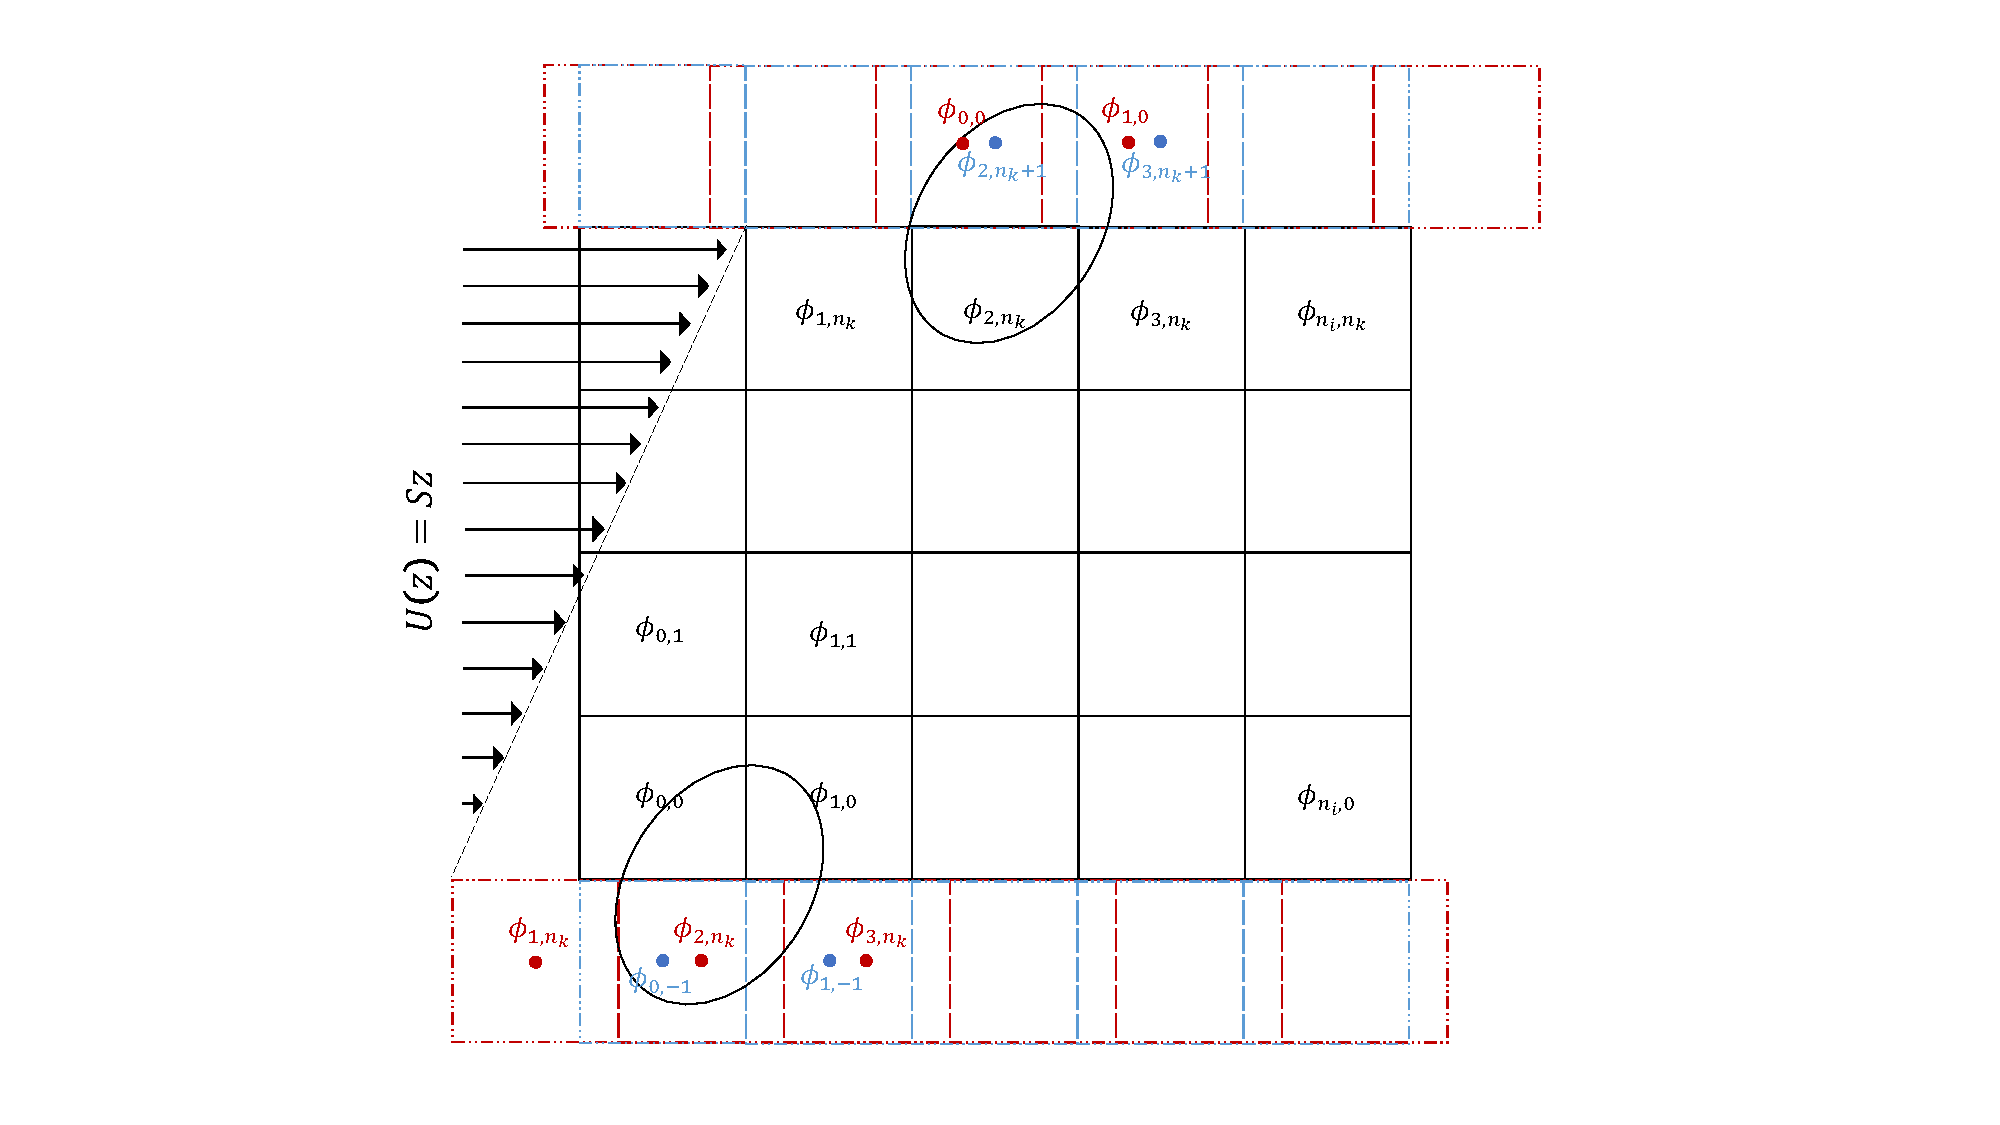
\includegraphics[scale=0.6]{figures/discretisation_ShearBC.pdf}
   \caption{\label{discretisation} Discrétisation de la condition de cisaillement périodique. En bleu, l'espace virtuel étendu du maillage cartésien. En rouge, figuration de la condition de shear-periodicité.}
\end{figure} 

La condition de shear-periodicté nécessite de nombreuses interpolations au niveau de la frontière $\partial\omega_z$ (voir figure~\ref{discretisation}) et des erreurs peuvent survenir et dégrader considérablement les calculs si elles ne sont pas gérées correctement. \\

Pour une grandeur quelconque, on peut écrire une interpolation telle que (voir figure~\ref{discretisation}) :

\begin{align}
\phi_{i,n_k+1}&=a_0\lrb{t}\phi_{i',0}+a_1\lrb{t}\phi_{(i-1)',0}+.+a_{n_i}\lrb{t}\phi_{(i-n_i)',0}\label{interpol}\\
\phi_{i,-1}&=a_0\lrb{t}\phi_{i',n_k}+a_1\lrb{t}\phi_{(i+1)',n_k}+.+a_{n_i}\lrb{t}\phi_{(i+n_i)',n_k}\label{interpol2}
\end{align}

Avec $i'=i\%n_i$ pour prendre le compte la périodicité selon $x$. Dans la suite, la notation $i'$ est abandonnée pour plus de lisibilité. 

\begin{align}
\phi_{i,n_k+1}&=\sum_{j\in n_i} a_j\lrb{t}\phi_{i-j,0}\label{interpol}\\
\phi_{i,-1}&=\sum_{j\in n_{i}}a_j\lrb{t}\phi_{i+j,n_k}\label{interpol2}
\end{align}
 
Les coefficients $a_j$ dépendront alors de l'interpolation choisie (régression linéaire, interpolation d'ordre supérieur etc.). Le décalage spatial étant fonction du temps, ces coefficients changent à chaque pas de temps pour satisfaire la condition \eqref{shear_perio} et satisfont la condition suivante :

\begin{align}
\sum_{j\in n_{i}} a_j\lrb{t}&=1\label{coef}
\end{align}


Dans le cas d'une maille diphasique, les grandeurs principales de l'écoulement sont résolues sous forme monofluide : $\phi=\sum_{k\in[l,v]}\phi_kI_k$ où $I_k$ est l'indicatrice de phase qui vaut 1 dans la phase $k$, et qui varie entre $0$ et $1$ dans les mailles diphasiques. L'interpolation d'une grandeur monofluide s'écrit alors :
\begin{align}
\phi^{i,n_k+1}&=I^{i,n_k+1}_v\phi^{i,n_k+1}_v+I^{i,n_k+1}_l\phi^{i,n_k+1}_l\label{monofluide}\\
\phi^{i,n_k+1}&=I^{i,n_k+1}_v\sum_{j\in n_{i}} a_j\lrb{t}\phi^{i-j,0}_v+I^{i,n_k+1}_l\sum_{j\in n_{i}} a_j\lrb{t}\phi^{i-j,0}_l\\
\phi^{i,n_k+1}&=\sum_{j\in n_{i}} a_j\lrb{t}\lrb{\phi^{i-j,0}_vI^{i,n_k+1}_v+\phi^{i-j,0}_lI^{i,n_k+1}_l}\\
\phi^{i,n_k+1}&\neq \sum_{j\in n_{i}} a_j\lrb{t}\phi_{i-j,0}\label{monofluide2}
\end{align}

A noter que numériquement, on connait à chaque instant la fonction indicatrice de phase et la courbure exacte (y compris dans les mailles ``fantômes'' ). Dans les expressions ci-dessus, on connait donc $I^{i,n_k+1}_v$, $I^{i,-1}_v$ car TrioIJK utilise un domaine étendu pour gérer la périodicité des interfaces. Les interfaces sont donc dupliquées au niveau des conditions périodiques, et l'indicatrice comme la courbure peuvent alors être calculées précisement aux éléments (y compris fantômes). 

En revanche, l'expression~\eqref{monofluide2} montre que, pour les grandeurs monofluides, il faut passer par une interpolation non triviale. On ne peut pas interpoler directement les grandeurs monofluides, et malheureusement, les grandeurs phasiques $\phi_v$ et $\phi_l$ sont inconnues (à l'exception des propriétés physiques de l'écoulement lorsqu'elles sont constantes par phase). La reconstruction des grandeurs phasiques par extrapolation de la variable monofluide pourrait être envisageable si le processus d'extrapolation nécessitait une puissance de calcul limitée, mais une telle solution est difficile à mettre en oeuvre. A noter que l'interpolation des grandeurs monofluides est un enjeu d'autant plus important pour les variables présentant un saut à l'interface (pression, densité, viscosité). 

\subsubsection{Interpolation des propriétés physiques constantes par phase}

Pour les propriétés thermodynamiques, constantes par phase, la reconstruction de la grandeur monofluide est triviale dès lors que l'on connait la fonction indicatrice dans les mailles fantômes. On écrit : 

\begin{align}
\rho_{i,n_k+1}&=\rho_lI^l_{i,n_k+1}+\rho_vI^v_{i,n_k+1}\label{rho1}\\
\rho_{i,-1} &= \rho_lI^l_{i,-1}+\rho_vI^v_{i,-1}\label{rho2}\\
\mu_{i,n_k+1}&=\mu_lI^l_{i,n_k+1}+\mu_vI^v_{i,n_k+1}\\
\mu_{i,-1} &= \mu_lI^l_{i,-1}+\mu_vI^v_{i,-1}
\end{align}

\subsubsection{Interpolation de la vitesse}

Pour des conditions adiabatiques, la vitesse ne présente pas de saut à l'interface liquide/vapeur.
Néanmoins, on observe qu'interpoler séparemment $\rho$ et $\ve{U}$ n'assure pas la conservation de la quantité de mouvement $\rho\ve{U}$. 
Dans la suite, deux méthodes seront donc testées :
\begin{itemize}
\item Interpolation directe de la vitesse monofluide : 
\begin{align}
U_{i,n_k+1}&=\sum_{j\in n_i} a_j\lrb{t}U_{i-j,0}+\lrbb{\lrbb{U}}_{\partial\omega_z}\\
U_{i,-1}&=\sum_{j\in n_{i}}a_j\lrb{t}U_{i+j,n_k}-\lrbb{\lrbb{U}}_{\partial\omega_z}
\end{align}
\item Interpolation indirecte assurant la conservation de la quantité de mouvement :
\begin{align}
U_{i,n_k+1}&=\frac{1}{\rho_{i,n_k+1}}\sum_{j\in n_i} a_j\lrb{t}\lrbb{\rho U}_{i-j,0}+\lrbb{\lrbb{U}}_{\partial\omega_z}\label{consevqdm1}\\
U_{i,-1}&=\frac{1}{\rho_{i,-1}}\sum_{j\in n_{i}}a_j\lrb{t}\lrbb{\rho U}_{i+j,n_k}-\lrbb{\lrbb{U}}_{\partial\omega_z}\label{consevqdm2}
\end{align}
\end{itemize}


\subsubsection{Interpolation de la pression}

Pour la pression (qui n'est pas constante par phase, et qui présente néanmoins un saut à l'interface), la situation est plus complexe. Une manière de s'en sortir est de noter la relation de saut de contraintes à l'interface dans la direction normale à l'interface :
\begin{align}
P_v^{I}-P_l^{I}+\lrb{\tau_{l,n}-\tau_{v,n}}&=\sigma\kappa^{i,n_k+1}\label{laplace1}
\end{align}
$\tau_{l,n}$ et $\tau_{v,n}$ sont les parties déviatoriques du tenseur des contraintes projetée selon la normale à l'interface: $\tau_{l,n} = \mu_l\nabla\ve{u_l}.\ve{n^I}$. A l'ordre 1, cette relation exprimée aux éléments donne :

\begin{align}
P_v^{i,n_k+1}-P_l^{i,n_k+1}&=\sigma\kappa^{i,n_k+1}+\tau_{v,n}^{i,n_k+1}-\tau_{l,n}^{i,n_k+1}+O\lrb{x_I-x}\label{laplace1}\\
P_v^{j,0}-P_l^{j,0}&=\sigma\kappa^{j,0}+\tau_{v,n}^{j,0}-\tau_{l,n}^{j,0}+O\lrb{x_I-x}\label{laplace2}
\end{align}
où $x_I-x$ est la distance normale entre le centre des éléments (où sont calculées les pressions), et la position de l'interface.

Avec l'expression \eqref{monofluide}, on obtient :
\begin{align}
P^{i,n_k+1}&= P_v^{i,n_k+1}-I_l^{i, n_k+1}\sigma\kappa^{i,n_k+1}-I_l^{i, n_k+1}\lrb{\tau_{v,n}^{i,n_k+1}-\tau_{l,n}^{i,n_k+1}}+O\lrb{x_I-x}\\
P^{j,0}&= P_v^{j,0}-I_l^{i, 0}\sigma\kappa^{i,0}-I_l^{i, 0}\lrb{\tau_{v,n}^{i,0}-\tau_{l,n}^{i,0}}+O\lrb{x_I-x}\label{eq2}
\end{align}
Avec les expressions ~\eqref{interpol} ~\eqref{interpol2}  ~\eqref{eq2}, et ~\eqref{coef} on obtient :
\begin{align}
P^{i,n_k+1}=& \sum_{j\in n_{i}} a_j\lrb{t}P^{i-j,0}+ \sum_{j\in n_{i}} a_j \lrbb{\sigma\lrb{I_l^{i-j, 0}\kappa^{i-j,0}-I_l^{i, n_k+1}\kappa^{i,n_k+1}}}\nonumber\\
&+\sum_{j\in n_{i}} a_j \lrbb{I_l^{i-j, 0}\lrb{\tau_{v,n}^{i-j,0}-\tau_{l,n}^{i-j,0}}-I_l^{i, n_k+1}\lrb{\tau_{v,n}^{i, n_k+1}-\tau_{l,n}^{i, n_k+1}}}+O\lrb{x_I-x}\label{interpole_pression1}\\
P^{i,-1}= &\sum_{j\in n_{i}} a_j\lrb{t}P^{i+j,n_k}+ \sum_{j\in n_{i}} a_j\lrbb{\sigma\lrb{I_l^{i+j, n_k}\kappa^{i+j,n_k}-I_l^{i, -1}\kappa^{i,-1}}}\nonumber\\
&+\sum_{j\in n_{i}} a_j\lrbb{I_l^{i+j, n_k}\lrb{\tau_{v,n}^{i+j,n_k}-\tau_{l,n}^{i+j,n_k}}-I_l^{i, -1}\lrb{\tau_{v,n}^{i, -1}-\tau_{l,n}^{i, -1}}}+O\lrb{x_I-x}\label{interpole_pression2}
\end{align}
Le premier terme du membre de droite est alors une interpolation classique de la grandeur monofluide. Il ne nécessite pas de reconstruire les grandeurs phasiques. Le second membre, lui, traduit l'erreur commise lorsqu'on interpole directement les grandeurs monofluides, en raison de l'interpolation linéaire de la fonction indicatrice de phase et de la courbure. Ce second terme du membre a l'avantage de pouvoir être calculé numériquement. Il permet de corriger l'erreur la plus importante commise sur l'interpolation de la pression dans les mailles diphasiques. Le troisième terme est la contribution du saut de contrainte visqueuse à l'interface, lequel doit être faible en comparaison du saut lié à la tension de surface. De plus, les termes $\tau_l$ et $\tau_v$ ne sont pas connus par la résolution, et la reconstruction des vitesses phasiques à l'interface serait trop lourde, raison pour laquelle ce terme sera negligé par la suite. Si des problèmes d'interpolation persistent, peut-être faudra t-il se limiter à des cas $\mu_l=\mu_v$. Enfin, le dernier terme, $O\lrb{x_I-x}$ est la contribution à l'erreur d'interpolation liée au décalage entre la pression résolue aux éléments et les pressions interfaciales. Si des problèmes d'interpolation persistent, on pourrait envisager une montée en ordre de la méthode pour prendre en compte ce paramètre. 

En attendant, dans la suite de ce travail, on utilisera l'interpolation naïve :

\begin{align}
P^{i,n_k+1}&\approx \sum_{j\in n_{i}} a_j\lrb{t}P^{i-j,0}\label{interpole_pression1}\\
P^{i,-1}&\approx \sum_{j\in n_{i}} a_j\lrb{t}P^{i+j,n_k}\label{interpole_pression2}
\end{align}
  

\subsection{Conséquence sur la matrice de pression}

Dans TrioIJK, il faut résoudre une équation de Poisson de la forme :

\begin{align}
\nabla.\lrb{\frac{1}{\rho}\nabla P} = f
\end{align}

La discrétisation du terme à l'intérieur de la divergence se fait aux faces, avec une interpolation de la masse volumique qui peut être arithmétique ou harmonique. Pour l'exemple, on choisit la moyenne arithmétique. La discrétisation de l'opérateur divergence aux éléments se fait alors à partir du gradient exprimé aux faces. On obtient, pour l'exemple en 2D: 

\begin{align}
&\frac{1}{h_x^2}\frac{2}{\rho_{i+1,k}+\rho_{i,k}}P_{i+1,k}+\frac{1}{h_x^2}\frac{2}{\rho_{i-1,k}+\rho_{i,k}}P_{i-1,k}+\frac{1}{h_z^2}\frac{2}{\rho_{i,k+1}+\rho_{i,k}}P_{i,k+1}+\frac{1}{h_z^2}\frac{2}{\rho_{i,k-1}+\rho_{i,k}}P_{i,k-1}\\
&-\lrbb{\frac{1}{h_x^2}\lrb{\frac{2}{\rho_{i+1,k}+\rho_{i,k}}+\frac{2}{\rho_{i-1,k}+\rho_{i,k}}}+\frac{1}{h_z^2}\lrb{\frac{2}{\rho_{i,k+1}+\rho_{i,k}}+\frac{2}{\rho_{i,k-1}+\rho_{i,k}}}}P_{i,k}= f_{i,k}\nonumber
\end{align}

Pour simplifier, on note ensuite :

\begin{align}
\alpha_{i+1,k}P_{i+1,k}+&\alpha_{i,k}P_{i-1,k}+\gamma_{i,k+1}P_{i,k+1}+\gamma_{i,k}P_{i,k-1}-4\delta_{i,k}P_{i,k}= f_{i,k}\\
\alpha_{i,k}&=\frac{1}{h_x^2}\frac{2}{\rho_{i,k}+\rho_{i-1,k}}\\
\gamma_{i,k}&=\frac{1}{h_z^2}\frac{2}{\rho_{i,k}+\rho_{i,k-1}}\\
\delta_{i,k}&=\frac{1}{4}\lrbb{\frac{1}{h_x^2}\lrb{\frac{2}{\rho_{i+1,k}+\rho_{i,k}}+\frac{2}{\rho_{i-1,k}+\rho_{i,k}}}+\frac{1}{h_z^2}\lrb{\frac{2}{\rho_{i,k+1}+\rho_{i,k}}+\frac{2}{\rho_{i,k-1}+\rho_{i,k}}}}
\end{align}

En considérant les conditions périodiques et shear-periodiques, on peut écrire :
\begin{align}
\alpha_{0,k}&=\alpha_{n_i+1,k}\\
\alpha_{-1,k}&=\alpha_{n_i,k}\\
\gamma_{i,-1}&\neq\gamma_{i,n_k}\label{symet_condition}\\
\gamma_{i,0}&\neq\gamma_{i,n_k+1}\label{symet_condition2}
\end{align}


Avec les expressions \eqref{interpole_pression1} et \eqref{interpole_pression2}, on obtient :
\begin{align*}
\alpha_{i+1,0}P_{i+1,0}+\alpha_{i,0}P_{i-1,0}+\gamma_{i,1}P_{i,1}+\gamma_{i,0}\sum_{j\in n_{i}}a_jP_{i+j,n_k}-4\delta_{i,0}P_{i,0}&= f_{i,0}&\text{sur}\partial\omega_z^-\\
\alpha_{i+1,n_k} P_{i+1,n_k}+\alpha_{i,n_k}P_{i-1,n_k}+\gamma_{i,n_k+1}\sum_{j\in n_{i}}a_jP_{i-j,0}+\gamma_{i,n_k}P_{i,n_k-1}-4\delta_{i,n_k}P_{i,n_k} &=  f_{i,n_k} \text{sur }\partial\omega_z^+ \\ 
\alpha_{i+1,k}P_{i+1,k}+\alpha_{i,k}P_{i-1,k}+\gamma_{i,k+1}P_{i,k+1}+\gamma_{i,k}P_{i,k-1}-4\delta_{i,k}P_{i,k}&=f_{i,k}\quad\text{ailleurs}
\end{align*}

Le système résolu s'écrit alors :

\begin{align} 
V\mathbf{A}\mathbf{P}&=V\mathbf{f} \\
\mathbf{A}&=\begin{pmatrix} 
         -4\delta_{0,0}&\alpha_{1,0}&.&0&\gamma_{0,1}&.&0&\gamma_{0,0}a_0(t)&.&\gamma_{0,0}a_{n_i}(t) \\ 
         \alpha_{1,0}&-4\delta_{1,0}&.&0&0&.&0&\gamma_{1,0}a_1(t)&.&\gamma_{1,0}a_{0}(t) \\ 
         .&.&.&.&.&.&.&.&.&. \\ 
         \alpha_{0,0}&0&.&-4\delta_{n_i,0}&0&.&0&\gamma_{n_i,0}a_{n_i}(t)&.&\gamma_{n_i,0}a_{n_i-1}(t) \\ 
         \gamma_{0,1}&0&.&0&-4\delta_{0,1}&.&0&0&.&0 \\ 
         .&.&.&.&.&.&.&.&.&. \\ 
         0&0&.&0&0&.&-4\delta_{n_i,n_k-1}&0&.&\gamma_{n_i,n_k} \\ 
         \gamma_{0,n_k+1}a_{0}(t)&\gamma_{0,n_k+1}a_{n_i}(t)&.&\gamma_{0,n_k+1}a_{1}(t)&0&.&0&-4\delta_{0,n_k}&.&\alpha_{0,n_k} \\ 
         .&.&.&.&.&.&.&.&.&. \\ 
         \gamma_{n_i,n_k+1}a_{n_i}(t)&\gamma_{n_i,n_k+1}a_{n_i-1}(t)&.&\gamma_{n_i,n_k+1}a_{0}(t)&0&.&\gamma_{n_i,n_k}&\alpha_{0,n_k}&.&-4\delta_{n_i,n_k} \\ 
   \end{pmatrix} \\
\mathbf{P}&=\begin{pmatrix} 
         P_{0,0}\\ 
         P_{1,0}\\
          . \\
         P_{n_i,0}\\
         P_{0,1}\\
         . \\
         P_{n_i,n_k-1}\\
         P_{0, n_k}\\  
         .\\ 
         P_{n_i,n_k}
   \end{pmatrix} ; 
   \mathbf{f}=
      \begin{pmatrix} 
         f_{0,0}\\ 
         f_{1,0}\\
          . \\
         f_{n_i,0}\\
         f_{0,1}\\
         . \\
         f_{n_i,n_k-1}\\
         f_{0, n_k}\\  
         .\\ 
         f_{n_i,n_k}
   \end{pmatrix}
\end{align}
où $V=h_xh_z$, le volume de l'élément.


